\documentclass[]{report}
\usepackage{lmodern}
\usepackage{amssymb,amsmath}
\usepackage{ifxetex,ifluatex}
\usepackage{fixltx2e} % provides \textsubscript
\ifnum 0\ifxetex 1\fi\ifluatex 1\fi=0 % if pdftex
  \usepackage[T1]{fontenc}
  \usepackage[utf8]{inputenc}
\else % if luatex or xelatex
  \ifxetex
    \usepackage{mathspec}
  \else
    \usepackage{fontspec}
  \fi
  \defaultfontfeatures{Ligatures=TeX,Scale=MatchLowercase}
\fi
% use upquote if available, for straight quotes in verbatim environments
\IfFileExists{upquote.sty}{\usepackage{upquote}}{}
% use microtype if available
\IfFileExists{microtype.sty}{%
\usepackage[]{microtype}
\UseMicrotypeSet[protrusion]{basicmath} % disable protrusion for tt fonts
}{}
\PassOptionsToPackage{hyphens}{url} % url is loaded by hyperref
\usepackage[unicode=true]{hyperref}
\PassOptionsToPackage{usenames,dvipsnames}{color} % color is loaded by hyperref
\hypersetup{
            pdftitle={ABJ Syllabus},
            pdfauthor={Associação Brasileira de Jurimetria},
            colorlinks=true,
            linkcolor=Maroon,
            citecolor=Blue,
            urlcolor=Blue,
            breaklinks=true}
\urlstyle{same}  % don't use monospace font for urls
\usepackage{natbib}
\bibliographystyle{apalike}
\usepackage{longtable,booktabs}
% Fix footnotes in tables (requires footnote package)
\IfFileExists{footnote.sty}{\usepackage{footnote}\makesavenoteenv{long table}}{}
\usepackage{graphicx,grffile}
\makeatletter
\def\maxwidth{\ifdim\Gin@nat@width>\linewidth\linewidth\else\Gin@nat@width\fi}
\def\maxheight{\ifdim\Gin@nat@height>\textheight\textheight\else\Gin@nat@height\fi}
\makeatother
% Scale images if necessary, so that they will not overflow the page
% margins by default, and it is still possible to overwrite the defaults
% using explicit options in \includegraphics[width, height, ...]{}
\setkeys{Gin}{width=\maxwidth,height=\maxheight,keepaspectratio}
\IfFileExists{parskip.sty}{%
\usepackage{parskip}
}{% else
\setlength{\parindent}{0pt}
\setlength{\parskip}{6pt plus 2pt minus 1pt}
}
\setlength{\emergencystretch}{3em}  % prevent overfull lines
\providecommand{\tightlist}{%
  \setlength{\itemsep}{0pt}\setlength{\parskip}{0pt}}
\setcounter{secnumdepth}{5}
% Redefines (sub)paragraphs to behave more like sections
\ifx\paragraph\undefined\else
\let\oldparagraph\paragraph
\renewcommand{\paragraph}[1]{\oldparagraph{#1}\mbox{}}
\fi
\ifx\subparagraph\undefined\else
\let\oldsubparagraph\subparagraph
\renewcommand{\subparagraph}[1]{\oldsubparagraph{#1}\mbox{}}
\fi

% set default figure placement to htbp
\makeatletter
\def\fps@figure{htbp}
\makeatother

\usepackage[brazilian]{babel}
\usepackage[utf8]{inputenc}
\usepackage[T1]{fontenc}
\usepackage{lipsum}
\usepackage{fullwidth}
\usepackage{indentfirst}
\usepackage[left=2.5cm, right=2.5cm, top=4cm, bottom=3.8cm]{geometry}
\renewcommand{\familydefault}{\sfdefault}
\PassOptionsToPackage{dvipsnames}{xcolor}
\RequirePackage{xcolor} % [dvipsnames]
\definecolor{halfgray}{gray}{0.55} % chapter numbers will be semi transparent .5 .55 .6 .0
\definecolor{webgreen}{rgb}{0,.5,0}
\definecolor{webbrown}{rgb}{.6,0,0}
%\definecolor{Maroon}{cmyk}{0, 0.87, 0.68, 0.32}
%\definecolor{RoyalBlue}{cmyk}{1, 0.50, 0, 0}
%\definecolor{Black}{cmyk}{0, 0, 0, 0}
\usepackage{fancyhdr}
\usepackage{pdfpages}
\usepackage{amsmath}
\usepackage{graphicx}
\usepackage{listings}
\usepackage{enumitem}
\usepackage{setspace}
\usepackage{spverbatim}
\usepackage{lipsum}
\usepackage{natbib}
\usepackage{longtable}
\usepackage{booktabs}
\usepackage{background}

\newcommand{\prestadorEmpresaFoot}{Associação Brasileira de Jurimetria}
\newcommand{\prestadorEmpresa}{Associação Brasileira de Jurimetria}
\newcommand{\prestadorRepr}{Marcelo Guedes Nunes}
\newcommand{\prestadorEnderecoFoot}{Rua Gomes de Carvalho, 1356, 2º andar. CEP 04547-005 - São Paulo, SP, Brasil.}
\newcommand{\prestadorEndereco}{Rua Gomes de Carvalho, 1356, 2º andar}
\newcommand{\prestadorEnderecoComp}{CEP 04547-005 - São Paulo, SP, Brasil}
\newcommand{\prestadorSite}{\url{http://abj.org.br}}
\newcommand{\prestadorEmail}{contato@abj.org.br}
% \includegraphics[trim=left bottom right top, clip]{file}
\newcommand{\logo}{\includegraphics[width=0.21\textwidth, trim=0cm 0cm 0cm 11.1cm, clip]{imgs/logo_abj.png}}

\newcommand{\tipoTrabalho}{}
\newcommand{\numero}{XXX}

\newcommand{\clienteEmpresa}{XXX}
\newcommand{\clienteEndereco}{XXX}
\newcommand{\clienteEnderecoComp}{XXX}
\newcommand{\clienteRepr}{XXX}
\newcommand{\clienteEmail}{XXX}

% \fancypagestyle{firststyle}
% {
%     \pagestyle{fancy}
%     \lhead{\thepage}
%     \chead{}
%     \rhead{\logo{}}
%     \cfoot{
%         \footnotesize{\prestadorEmpresaFoot{}} \\
%         \footnotesize{\prestadorEnderecoFoot{}} \\
%         \footnotesize{\prestadorSite{}}
%     }
%     \renewcommand{\headrulewidth}{0.5pt}
%     \renewcommand{\footrulewidth}{0.5pt}
%     \setlength{\headsep}{.5in}
% }
%
% \pagestyle{firststyle}

\setlength{\parindent}{2em}
% \setlength{\parskip}{1em}
% \renewcommand{\baselinestretch}{1.2}
% % \usepackage{palatino}
% \renewcommand{\familydefault}{\sfdefault} % sans serif
% \fontfamily{ppl}\selectfont

%\renewcommand{\baselinestretch}{1.4}

\backgroundsetup{
scale=1,
angle=0,
opacity=1,
color=black,
contents={\begin{tikzpicture}[remember picture,overlay]
\node at ([xshift=-4.35cm,yshift=-2.5cm] current page.north east) % Adjust the position of the logo.
{\logo}; % logo goes here
\end{tikzpicture}}
}

\usepackage{float}
\let\origfigure\figure
\let\endorigfigure\endfigure
\renewenvironment{figure}[1][2] {
    \expandafter\origfigure\expandafter[H]
} {
    \endorigfigure
}

\title{ABJ Syllabus}
\author{Associação Brasileira de Jurimetria}
\date{03 de abril de 2018}

\usepackage{amsthm}
\newtheorem{theorem}{Theorem}[chapter]
\newtheorem{lemma}{Lemma}[chapter]
\theoremstyle{definition}
\newtheorem{definition}{Definition}[chapter]
\newtheorem{corollary}{Corollary}[chapter]
\newtheorem{proposition}{Proposition}[chapter]
\theoremstyle{definition}
\newtheorem{example}{Example}[chapter]
\theoremstyle{definition}
\newtheorem{exercise}{Exercise}[chapter]
\theoremstyle{remark}
\newtheorem*{remark}{Remark}
\newtheorem*{solution}{Solution}
\begin{document}
\maketitle

{
\hypersetup{linkcolor=black}
\setcounter{tocdepth}{2}
\tableofcontents
}
\listoftables
\listoffigures
\chapter{Introduction}\label{introducao-2}

Para que o seu \texttt{bookdown} funcione tanto na web quanto no pdf,
você deve evitar usar marcadores que dependem do contexto.

Para fazer citações você deve usar \citep{Weinstein1997} ou
\citet{Weinstein1997}. Isso também funciona pra pacotes \citep{R-base}
ou \citet{R-base}. Para criar uma figura, é preferível que você use o
\texttt{print} padrão do \texttt{knitr}. A label do gráfico será
\texttt{fig:label-do-chunk}. Você pode citar fazendo
\ref{fig:label-do-chunk}.

\begin{figure}
\centering
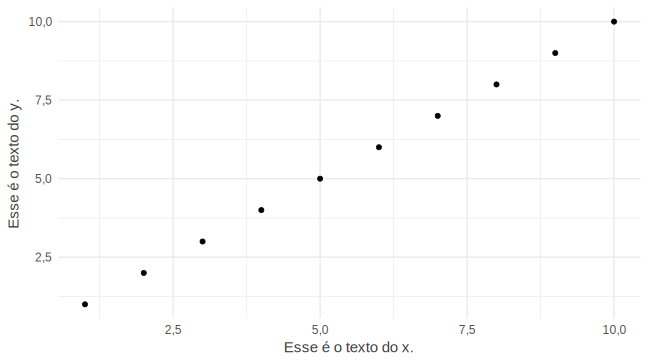
\includegraphics{bookdown_files/figure-latex/label-do-chunk-1.pdf}
\caption{\label{fig:label-do-chunk}Este é um gráfico.}
\end{figure}

Se você precisar importar uma imagem de fora do R, é melhor que você
faça \texttt{!{[}{]}()}, a despeito do que diz o Yihui.

Se você estiver com muita vontade de seguir os ensinamentos do mestre,
você pode usa o \texttt{knitr::include\_graphics}, mas vai precisar
setar \texttt{dpi\ =\ NA}.

\begin{figure}

{\centering \includegraphics{imgs/logo_abj} 

}

\caption{The RStudio addin to help input LaTeX math.}\label{fig:mathquill}
\end{figure}

Essa forma tem duas vantagens:

\begin{enumerate}
\def\labelenumi{\arabic{enumi}.}
\tightlist
\item
  A label fica no mesmo formato das demais.
\item
  Você pode setar o \texttt{fig.height} e o \texttt{fig.width}.
\end{enumerate}

Escolhendo qualquer uma das formas, não é uma boa importar imagens que
vieram de dentro de pastas. Você terá problemas com o \texttt{path} dos
arquivos. O \texttt{bookdown} não copia as pastas pra dentro do
\texttt{\_book}, você precisará fazer isso manualmente.

Outro tipo de referência interessante é a referência a subseções. Você
pode usar {[}essa sintaxe{]}{[}objetivos{]} pra ir pra seção de
objetivos. Você também pode usar \ref{objetivos}, contanto que tenha
colocado \{\#objetivos\} na definição da seção.

Por fim, pra inserir tabelas, use apenas \texttt{kable}. Esse
\texttt{book} sabe o que fazer dependendo do \texttt{output}.

\begin{table}[H]
\centering
\begin{tabular}{rrrrrrrrrrr}
  \hline
mpg & cyl & disp & hp & drat & wt & qsec & vs & am & gear & carb \\ 
  \hline
21,00 & 6,00 & 160,00 & 110,00 & 3,90 & 2,62 & 16,46 & 0,00 & 1,00 & 4,00 & 4,00 \\ 
  21,00 & 6,00 & 160,00 & 110,00 & 3,90 & 2,88 & 17,02 & 0,00 & 1,00 & 4,00 & 4,00 \\ 
  22,80 & 4,00 & 108,00 & 93,00 & 3,85 & 2,32 & 18,61 & 1,00 & 1,00 & 4,00 & 1,00 \\ 
  21,40 & 6,00 & 258,00 & 110,00 & 3,08 & 3,21 & 19,44 & 1,00 & 0,00 & 3,00 & 1,00 \\ 
  18,70 & 8,00 & 360,00 & 175,00 & 3,15 & 3,44 & 17,02 & 0,00 & 0,00 & 3,00 & 2,00 \\ 
   \hline
\end{tabular}
\caption{Essa é uma tabela.} 
\end{table}

\chapter{About this book}\label{about-this-book}

O conteúdo desse livro será escrito parte em portugês e parte em inglês.
A justificativa dos autores sempre será ``escrevi como me senti mais
confortável''.

How to cite an article \citep{Weinstein1997}. How to cite a package
\citep{R-bookdown}.

\section{Who we are}\label{who-we-are}

\section{What do we look for on our
readings}\label{what-do-we-look-for-on-our-readings}

\section{How to read this book}\label{how-to-read-this-book}

\chapter{Machine learning}\label{machine-learning}

\section{Legal docket-entry classification: where machine learning
stumbles}\label{legal-docket-entry-classification-where-machine-learning-stumbles}

\begin{itemize}
\tightlist
\item
  Author: Ramesh Nallapati, Christopher D. Manning
\item
  Link: \url{https://nlp.stanford.edu/pubs/D08-1046.pdf}
\item
  keywords: docket-entry, classification
\end{itemize}

In US courts, the relevant events in a case are summarized
chronologically as brief descriptions. These descriptions are called
docket-entries. It is a hard problem to automatically classify these
docket-entries by type. The paper studies how to classify whether, in
given docket-entry for ``summary judgement'' (OSJ), the OSJ was granted
or not. The paper finds that standard models, such as SVM based on
bag-of-words, don't have optimal classification. A model that takes into
account propositional logic has a higher predictive power.

Data: 5,595 docket-entries that were hand-labeled by a single legal
expert as OSJ or not OSJ. The 1,848 OSJ docket-entries were labeled as
granted or not granted.

Preprocessing: Removed punctuation, casefold and stopwords. Performed
stemming.

Standard SVM: Bag-of-words for unigrams and bigrams on the whole data.
Several features are correlated to the label but have no predictive
power, e.g., ``opinion'', ``memorandum'', \(\ldots\)

SVM on hand-picked features: Bag-of-words for unigrams selected by
humans. Better performance.

Problem: While SVM is based on an additive model, propositional logics
has a different structure. Example: although ``moot'' and ``not'' have
negative values, ``not moot'' has a positive value.

New classifier: A deterministic propositional model based on expert. An
entry is positive if any sentence in the description is positive. A
sentence is positive if the multiplication of the unigram values in the
sentence is positive. Although naive, performs better than SVM.

Challenge: Build classifiers that capture semantics of natural language.
The difficult part is that the semantics is defined by non-linear
associations between words that are distant from one another (in
different sentences).

\chapter{Statistics}\label{statistics}

\section{Questionnaires}\label{questionnaires}

\subsection{Questionnaire design}\label{questionnaire-design}

\begin{itemize}
\tightlist
\item
  Author: U.S. Survey Research
\item
  Link:
  \url{http://www.pewresearch.org/methodology/u-s-survey-research/questionnaire-design/}
\item
  keywords: questionnaire design
\end{itemize}

Considerable differences between choices in open- and closed-ended
questions. In closed-ended questions, respondents rarely choose the
``others'' alternative, even when they agree with it. A common practice
is to perform a pilot study with open-ended alternatives followed by a
definitive study with closed-ended questions.

Number of alternatives should be generally be kept relatively small.
Otherwise, lack of memory and attention might generate errors. Many
alternatives are ok for a question such that the respondent already
knows the answer, e.g., ``what is your religion?''

The order of the alternatives should generally be randomized. In case of
ordinal variables, the order should be randomized between top to bottom
and bottom to top. This does not avoid the placement biase, but dilutes
it accross the alternatives.

Questions should be asked in a clear and direct fashion. Language should
be as simple as possible and never more sophisticated than the education
level of respondents. One question should be asked at a time. Questions
that try to approach two or more concepts at a time should be avoided.

There is a bias in which people generally choose the option ``agree'' in
questions with the alternatives ``agree'' and ``disagree''.

Wording of answers strongly influences the responses. Words that are too
positive or negative can bias the answer. The context provided in the
question also changes the answer.

Respondents have a bias towards ``socially desirable'' answers, e.g.,
drug usage is often understated and charity overstated. Alternatives
that describe a motivation can often make it easier for a person to
choose a socially undesirable response.

The order of the questions affects the answers. Previous questions can
be used as context for later questions. Questions should be grouped by
topic and unfolded in a logical order. Interesting and engaging
questions should be mixed with less interesting questions.

Pilot test: Useful when testing new questions. An application of the
questionnaire.

Focus groups: Several people debate the survey topic. Useful to
understand what topics are hot, how they understand these topics and how
they interpret the questions. Moderator typically asks broad questions.

\chapter{Law and Economics}\label{law-and-economics}

\section{Empirical evaluation of law: The dream and the
nightmare}\label{empirical-evaluation-of-law-the-dream-and-the-nightmare}

\citep{donohue2015empirical}

\section{The Priest-Klein hypotheses: Proofs and
generality}\label{the-priest-klein-hypotheses-proofs-and-generality}

\begin{itemize}
\tightlist
\item
  Author: Yoon-Ho Alex Lee, Daniel Klerman
\item
  Link:
  \url{https://ac.els-cdn.com/S0144818816300291/1-s2.0-S0144818816300291-main.pdf?_tid=353ca924-b0e5-11e7-b7da-00000aab0f6c\&acdnat=1507988594_6b1e434199243ddb26cf42d6184017b4}
\item
  Year: 2016
\item
  keywords: litigation, selection, priest and klein, decision theory,
  game theory
\end{itemize}

\citep{priest1984selection} is very famous for the hypothesized
``tendency toward 50 percent plaintiff victories''.
\citep{lee2016priest} argues that the original paper is not very clear
in a mathematical sense, so it demands a serious formalization. The main
goal of this paper is to prove or disprove the P\&K hypothesis using a
tough mathematical formulation.

According to the authors, there are 6 hypotheses attributable to Priest
and Klein:

\begin{enumerate}
\def\labelenumi{\arabic{enumi}.}
\item
  Disputes selected for litigation (as opposed to settlement) will not
  constitute a random sample nor a representative sample of all
  disputes.
\item
  As the parties error diminishes and the litigation rates declines, the
  proportion of plaintiff victories approaches 50\%.
\item
  Regardless of legal standard, the plaintiff trial win rate exhibit ``a
  strong bias toward fifty percent'' as compared to the plaintiff trial
  win rate that would be observerd if every case went to trial.
\item
  If the defendant would lose more from an adverse judgement than the
  plaintiff would gain, then the plaintiff will win less than fifty
  percent of the litigated cases. Conversely, if the plaintiff has more
  to gain, then the plaintiff will win more than fifty percent of the
  cases.
\item
  The plaintiff trial win rate will be unrelated to the shape of the
  distribution of disputes. This hypothesis is about the plaintiff win
  rate in the limit as the parties become increasingly accurate in
  predicting trial outcomes.
\item
  Because selection effects are strong, no inferences can be made about
  the law or legal decisionmakers from the plaintiff win rate. Rather,
  ``the proportion of observerd plaintiff victores will tend to remains
  constant''.
\end{enumerate}

The authors prove or disprove those hypothesis by using a mathematical
formulation of the Priest and Klein setting. They use a particular one,
but through this text i'll reproduce their arguments using a similar
version proposed on an unpublished papaer by \citep{gelbach2016reduced}.

Almost every model for litigation starts with

\begin{itemize}
\tightlist
\item
  \(Q_p\), the probability of plaintiff victory atributed by the
  plaintiff (possibly random).
\item
  \(Q_d\), the probability of plaintiff victory atributed by the
  defendant (possibly random).
\item
  \(c_p\), the cost of litigation for the plaintiff.
\item
  \(c_d\), the cost of litigation for the defendant (possibly null).
\item
  \(s_p\), the cost of pre-processual settlement for the plaintiff.
\item
  \(s_d\), the cost of pre-processual settlement for the defendant.
\item
  A joint probability distribution on \((Q_p, Q_d)\)
\item
  A bernoulli random variable \(\mathcal{L}\) indicating whether or not
  the ltigation ocurred.
\item
  A bernoulli random variable \(\mathcal{P}\) indicating whether or not
  the plaintiff won.
\item
  A litigation rule
  \(L(q_p, q_d) = \mathbb{E}[\mathcal{L}|Q_d = q_d, Q_p = q_p]\) that
  gives the probability of litigation given the parties subjective
  belief.
\item
  The probability of win of the plaintiff when the litigation occurred
  \(P(q_d, q_d) = \mathbb{E}[\mathcal{P}|\mathcal{L}=1, Q_d = q_d, Q_p = q_p]\)
\end{itemize}

Priest and Klein paper adds some parameters to the usual setting: \(J\),
\(\alpha\), \(Y\), \(Y_d\) and \(Y_p\). \(Y\) is a random quantity that
indicates the true quality of the case and \(Y_d\) and \(Y_p\) are noisy
approximations of \(Y\) that are accessible for the parties. \(Y\) and
\(y^*\) are numerical representations of lawsuit's variability and court
decision criterion: if \(Y > y^*\), some threshold number defined by the
court, the plaintiff wins the case.

Encoding costs to the decision process, \(J\) is the expected cost to
the defendant if the plaintiff wins and \(J_p = \alpha J\) is the
benefits for the plaintiff (if she wins). \(\alpha\) moderates the
stakes. If \(\alpha = 1\), the stakes are symmetric, and \(\alpha\)
\(>\) or \(<\) than 1 indicates stakes that favors plaintffs and
defendants, respectively.

Two important quantities for the selection of cases for litigation are

\begin{enumerate}
\def\labelenumi{\arabic{enumi}.}
\tightlist
\item
  Plaintiff's expected win: \(q_pJ\alpha-c_p\)
\item
  Defendant's expected cost: \(q_dJ+c_d\)
\end{enumerate}

Those quantities are important because \citep{priest1984selection}
states that " \(q_pJ\alpha-c_p+s_p > q_dJ+c_d-s_d\) is a sufficient
condition for litigation``. The intuition behind this statement comes
from the description of those quantitites:

\begin{enumerate}
\def\labelenumi{\arabic{enumi}.}
\tightlist
\item
  \(q_dJ+c_d-s_d\) is the largest amount the defendant is willing to
  pay. There's a lawsuit when the plaititff thinks that this number is
  too small.
\item
  \(q_pJ\alpha-c_p+s_p\) is the lowest amount the defendant is willing
  to receive. There's a lawsuit when the plaititff defendant thinks that
  this number is too high.
\end{enumerate}

\citep{lee2016priest} claims that \citep{priest1984selection} uses this
condition not only as sufficient but also as a necessary one, altough
neither they explictly mention why nor I could find it explictly noted
on the original paper. Through this text I'll act as if this was true.

Doing some algebra we get that the litigation condition is equivalent to

\[ q_p > \frac{q_d}{\alpha} +  \frac{c_p + c_d - s_d-s_p}{\alpha J} \]

That will therefore be called Landes-Posner-Gould (LPG) condition, as
the authors did.

To follow the demonstrations on the paper, we only need to add
probability measures on the setting defined above. Different from
\citep{priest1984selection}, here the parties also have opinions on
\(Y\). The setting may be resumed on a small set of claims:

\begin{itemize}
\tightlist
\item
  \(Y \sim N(0,1)\) and \(\epsilon_p \sim \epsilon_d \sim N(0,\sigma)\),
  all independent.
\item
  \(Y_p = Y + \epsilon_p\) and \(Y_d = Y + \epsilon_d\).
\item
  The parties has prior beliefs on \(Y\) that are represented by \(g_p\)
  and \(g_d\), respectively.
\end{itemize}

The decision procedures of the parties follows the following steps:

\begin{enumerate}
\def\labelenumi{\arabic{enumi}.}
\tightlist
\item
  Both of them have prior opinions on the probability of a plaitiff's
  win given by \(G_p(Y < y^*)\) and \(G_d(Y < y^*)\).
\item
  They observe a noisy measure of \(Y\), \(Y_p\) and \(Y_d\).
\item
  They updates their prior beliefs using using the normal likelihood and
  the \(g_p\) prior.
\item
  Their posteriors, \(Y|Y_p = y_p\) and \(Y|Y_d=y_d\), produce posetrior
  probabilities of plaitinff's win, given by
  \(\mathbb{P}(Y \leq y^*|Y_i = y_i)\), \(i \in \{p,d\}\).
\item
  LPG's selects cases for litigation based on the posterior
  probabilities.
\end{enumerate}

The original paper doesn't tell this story but gives the posterior
inferences:

\[ q_p = \Phi\left(\frac{Y_p - y^*}{\sigma}\right) \text{ and }q_d = \Phi\left(\frac{Y_d-y^*}{\sigma}\right)\]

This is equivalent as setting \(g_p \propto 1\) on the real line. In
this setting, \(Y_p ~ N(Y, \sigma)\), with a known \(\sigma\), so that
the posterior inference on \(Y\) is equivalent to doing normal bayesian
inference on a sample of size one and a flat prior. This gives us that
\(Y|Y_p=y_p \sim N(Y_p, \sigma)\), and then
\(\mathbb{P}(Y \leq y^*|Y_i = y_i) = \Phi\left(\frac{y^*-Y_i}{\sigma}\right)\).

Until now, nothing has been said on the population distribution of
\(Y\). \citep{priest1984selection} do not On that case, the probability
of plaintiff win is given by

\[W(y|y^*) = \int \int_{R(y,y^*)}\left(\frac{1}{\sqrt{2\pi\sigma^2}}\right)^2f_{Q_p}(u)f_{Q_d}(v)dudv\]

where
\(R(y, y^*) = \left\{u,v: \Phi\left(\frac{y+u-y^*}{\sigma}\right) - \Phi\left(\frac{y+v - y^*}{\sigma}\right) > K\right\}\)

\chapter{Theory of Law}\label{theory-of-law}

\section{Jurimetrics: The Methodology of Legal
Inquiry}\label{jurimetrics-the-methodology-of-legal-inquiry}

\begin{itemize}
\tightlist
\item
  Author: Lee Loevinger
\item
  Link:
  \url{http://scholarship.law.duke.edu/cgi/viewcontent.cgi?article=2945\&context=lcp}
\item
  Year: 1959
\item
  keywords: jurimetrics, theory of the law, lee loevinger, science
\end{itemize}

\citep{loevinger1963jurimetrics} define Jurimetria como aplicação de
metodologia científica no campo da lei. O autor deixa claro que existe
um desconforto na definição pura de qualquer área do conhecimento, mas
sempre é possível dizer pragmaticamente o que os praticantes de um certo
estudo fazem. Nas palavras do próprio Lee, o que um jurimetrista faz é

\begin{quote}
Jurimetrics is concerned with such matters as the quantitative analysis
of judicial behavior, the application of communication and information
theory to legal expression, the use of mathematical logic in law, the
retrieval of legal data by electronic and mechanical means, and the
formulation of a calculus of legal predictability. Jurisprudence is
primarily an undertaking of rationalism; jurimetrics is an effort to
utilize the methods of science in the field of law.
\end{quote}

Depois ele dá uns exemplos que vou discutir quando eu tiver mais tempo.

\bibliography{bibliography/book.bib,bibliography/packages.bib}

\end{document}
